\chapter{Introduction}\label{introduction}

\section{Motivation}\label{motivation}

\settowidth{\epigraphwidth}{Wonderful life : the Burgess Shale and the nature of history}
\epigraph{%
Without hesitation or ambiguity, and fully mindful of such paleontological wonders as large dinosaurs andAfrican ape-men, I state that the invertebrates of the Burgess Shale, found high in the Canadian Rockies in YohoNational Park, on the eastern border of British Columbia, are the world's most important animal fossils. Modern multicellular animals make their first uncontested appearance in the fossil record some 570 million years ago--and with a bang, not a protracted crescendo.}%
{\textit{\\Wonderful life : the Burgess Shale and the nature of history}\\\textsc{Stephen Jay Gould}}

Motivation is to understand the onset of evolution; how robust, interesting, adaptive evolution can be started and undergo self-improvement in the non-living world.

Our belief is that the evolution of evolution can and will emerge under certain conditions, and that a bottoms-up approach emergent approach will be more successful than the predominant design-driven top-down approach today.

Evolution in the Spencerian sense of progressive improvement, rather than necessarily any particular mechanism (e.g., evolution by natural selection). A change of population distribution over time--but if just purely distributive (sensu \autocite{Bourrat2015}), rather than transformative, not very interesting

Abstract idea, different from mechanisms such as ENS (grounded perhaps inseparably in biology) e.g., ``Darwin's theory of evolution by natural selection is restricted in scope. One sense in which it is restricted is that it refers to organisms.'' \autocite{Griesemer2005}

ENS as ``a theory of descent with modification''

Life (see later) provides the canonical example of ``interesting''; approaching life's creativity in an artificial system would be quite something.  Hope to see robustnes,  evolvability, novelty.

Natural selection as mechanism for adaptation (in biological sense). Assume that adaptation in this sense is useful concept for CS

Simple ongoing evolution is not the same as creative or interesting evolution; current state-of-the-art insufficient and unsatisfying. \autocite{Bourrat2015} makes a related distinction between distributive and transformative forms of evolution, where distributive evolution sees simply a change in population distribution without the generation of novelties or new elements characteristic of transformative evolution. The fundamental open problem is how to achieve transformative evolution in artificial systems.

\emph{A copy mechanism with adjustable fidelity can auto-adjust for example to changing environmental conditions.}

\begin{itemize}
	\item
	      Not same as ENS--that explains natural processes; our goal is to achieve something that is as interesting in a different domain
	\item 
	      Not same as EAs--EAs have exogenous fitness, not open-ended (search through a fixed space, cannot surprise (e.g., \autocite{Nellis2014})
	\item  
	      Not same as approach where take ideas from biology and evaluate for different purpose (e.g., in EAs, island populations, GRNs (e.g., L-systems), Lamarkian learning, co-evolution, evolutionary transitions (cooperation and mediation in \autocite{Defaweux:2005fk}\ldots{}). All seem to follow model of currently we use these tools, biology has something we don't have, let's try it\ldots{}
	\item
	      Not the same as most type of Alife, where evolution is not the subject of the research but rather a tool or mechanism towards some other goal (canonically, creating artificial life.)
\end{itemize}

Alternatives to ``evolution''?

\begin{itemize}
	\item Lower bound is random search--not good enough
	\item Upper bound is unknown--but ENS is the current gold standard for self-improving complex systems
	\item A good result would be `interesting' forms
\end{itemize}

\subsection{Why important?}\label{why-important}

\begin{itemize}
	\item Application to engineering -- alternative to EC approaches -- self-optimizing mechanism -- EvoEvo for EAs
	\item In itself--one of grand challenges of Alife \autocite{Bedau:2000mi}
	\item Possibly some application to other related fields (see \cref{relationships-with-other-fields})
\end{itemize}

\subsection{Life, the gold standard}

\subsubsection{Living organisms are supremely well suited to their environments, and can adapt to environmental changes}
\label{living-organisms-are-supremely-well-suited-to-their-environments-and-can-adapt-to-environmental-changes}

Adaptation of organisms to their environments occurs in the main on two
different time-scales.

Evolution by \gls{naturalselection} acts over a period of generations on
populations of individual organisms. Changes are therefore relatively
gradual, and many generations can pass before a change such as a
beneficial mutation becomes ubiquitous in a population (\eg 300-500
generations for targeted modifications in lactose processing in
\emph{E. coli} \autocite{Dekel:2005fk}. In contrast, gene regulatory
effects act during the life cycle of a single individual, either during
development to affect morphology, or during the adult lifespan in
reaction to seasonal or other environmental cues. These
regulation-driven changes are not in themselves heritable, but they can
be assimilated back into the population by influencing the organisms
fitness under natural selection (\eg,
\autocite{Baldwin:1896ly,Dennett:2003ve,Paenke:2009xe,Paenke:2007ve}).

Similar effects can be seen by another adaptive mechanism that operates
on individuals during their lifespan: learning, where behavioural
adaptions can also lead to genetic change
(\eg \autocite{Hinton:1987vy}.)

\subsubsection{Natural selection, acting on populations, is the primary driver for long-term adaptation}
\label{natural-selection-acting-on-populations-is-the-primary-driver-for-long-term-adaptation}

The year 2009 saw the celebration of the 150\textsuperscript{th}
anniversary of the publication of \emph{On the Origin of Species}, the
explanation of evolution by natural selection, with extensive coverage
in scientific and popular media. The terms are therefore fairly well
known to many people, but what exactly does \emph{natural selection}
mean? To quote from \autocite{Futuyama:1979tg}, \gls{naturalselection}
is the ``differential survival and reproduction of genotypes''.

Let's examine each of the components in this idea in turn:

Differential survival. Living organisms are constantly engaged in an
intimate relationship with their environments. Indeed, according to the
theory of \emph{autopoiesis} \autocite{Varela:1974qd}, organisms are
defined by this engagement: to be alive means maintaining oneself
against the surrounding environment. In general the more effectively the
organism is able to do this, the more likely it is to survive. However,
in practice survival for an individual may be affected by random events.
Scholarship winning students can be killed by drunk drivers. Sardines in
shoals flash and turn, yet sharks still manage to grab one or two from
the shoal effectively at random. Averaged over a population however
these chance events balance out; a succession of random trials leads to
a skewed distribution of fitness away from the less able.

\footnote{This introduces two significant differences between \glspl{ea}
	and biology: first, \glspl{ea} conduct a series of discrete trials of fitness,
	rather than a continuous evaluation. Second, fitness in an \gls{ea} is
	measured by an explicit \emph{objective function} whereas in biology
	fitness \emph{emerges dynamically} through continuous interaction with
the environment.}

Reproduction. In this sense, reproduction simply means inheritance. Only
those characteristics that can be passed on from one generation to the
next are relevant. One implication of this is that the only traits of an
organism that matter to natural selection are those that are apparent
while the organism can reproduce. Altruism and kin-selection, where an
individual acts to increase the fitness of a related individual, are
interesting for the light they shed on this implication.

Genotypes. An organism's \gls{genotype} is the heritable information
that defines an individual, of which the great majority is encoded in
DNA (some \emph{epigenetic} information is inherited through
DNA-methylation, maternal protein concentrations and other mechanisms.
However, generally DNA remains the primary source.)

How then does natural selection unfold in practice? Although an organism
is defined by its genotype, its survival is based not on the raw
genotype, but on the expression of the genotype--called the
\gls{phenotype}--that participates in the interaction with the
environment. There is not necessarily a direct one-to-one mapping
between genotype and phenotype; for example, environmental triggers
during development can switch the phenotype in different directions (a
phenomenon called \gls{polyphenism}.)

This indirect mapping enables a number of important mechanisms
significant to the operation of natural selection: first, changes in the
genotype (caused by mutations for example) may build up independent of
phenotype changes--the idea of \emph{neutral mutations}
\autocite{Ohta:1996vn,Ohta:2002ys,Ohta:1973kx}. Examples from studies
of RNA secondary structures (the physical folding of RNA molecules) show
that many closely-related RNA sequences can produce the same RNA folding
\autocite{Fontana:1993zn}. Adjacent changes often have little effect on
structure.

Second, by extension, \autocite{Gavrilets:1997qt} and
\autocite{Gravner:2007yd} have shown that in cases involving many gene
loci under well-defined conditions there is a path between viable
phenotypes that requires only neutral mutations.

Third, behaviours such as learning, rather than purely genetic
mechanisms, can influence the form of this \gls{gpmap} in combination
with natural selection, as illustrated by the Baldwin effect
\autocite{Baldwin:1896ly} and other examples of genetic assimilation
{[}\autocite{Hinton:1987vy};Siegal:2002qn;Waddington:1942jb{]}.

Finally, \glspl{grn} provide another mechanism to modify the \gls{gpmap}
and hence to guide natural selection.

\subsubsection{Novelties often arise from new regulatory connections rather than changes to genes}
\label{novelties-often-arise-from-new-regulatory-connections-rather-than-changes-to-genes}

\autocite{Prudhomme:2007ax} believe that evolutionary novelties more
commonly arise from changes or additions of regulatory
\emph{connections} than from the development of \emph{new} genes or
regulatory elements; that is, from changes to the network topology
rather than from additions to the network elements. The underlying
implication is that novelties are therefore new compositions of
pre-existing elements, rather than being constructed `\emph{de novo}',
and that production of novelties may be relatively rapid. Connection
changes may happen quickly; by comparison, new genes may take many generations.

\section{Problem}



\section{Approach and methods}\label{approach}

\begin{itemize}
	\item
	      Want to remove extraneous factors as factors introduce complications
	\item
	      Identification of necessary conditions vs contingent factors
	\item
	      Ideally minimal choices to be made or parameters to be chosen
\end{itemize}

Untangle the general from the biological in previous work. Emergent, self-improving, actionist (similar to Brooks in AI)

Much previous work aimed at understanding biology--assumes that domain.

\begin{figure}
	\begin{center}
		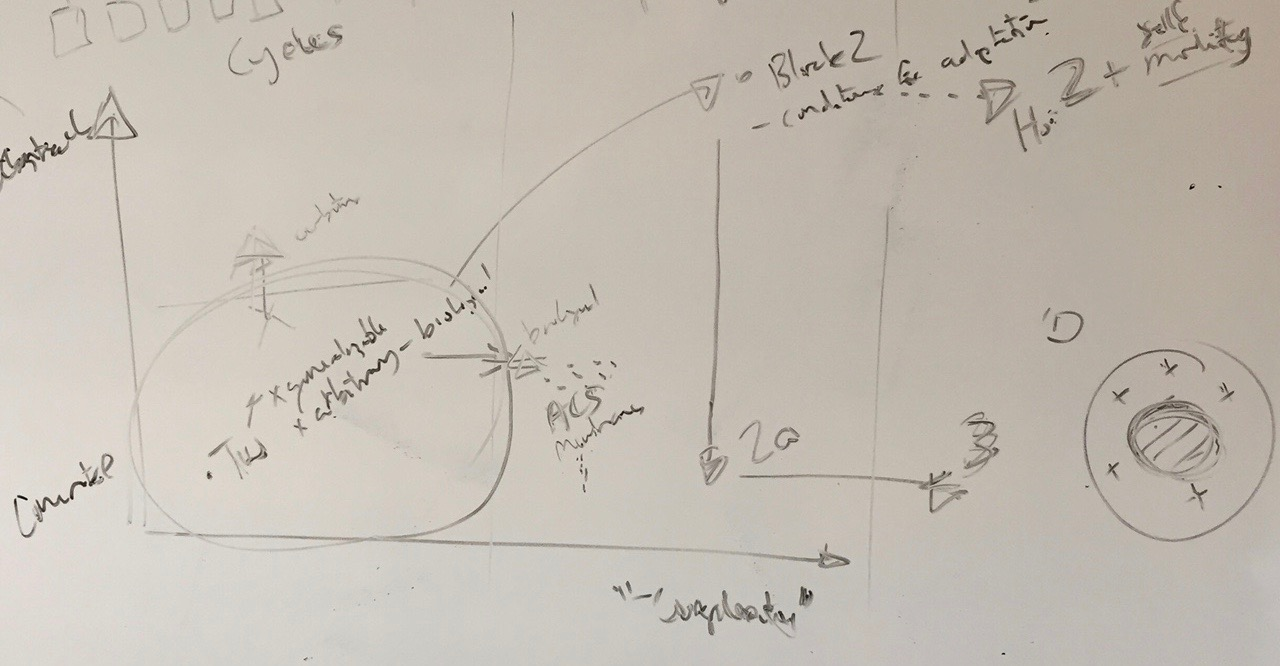
\includegraphics[width=\linewidth]{figures/approach}
	\end{center}
\end{figure}

\TODO{rewrite, properly mark quotations + references!}

The field of artificial life is synonymous with simulation
\autocite[chap.2]{Aicardi2010}. In other forms of science however
practitioners make use of a number of tools, including experiments,
mathematical models, thought experiments, and simulations.
Each method is well suited to some types of
questions, and inappropriate for others. Is the use of simulation
justified for our proposed investigation?

Simulations are becoming central to some disciplines in natural history.
Ecology--\glspl{abm} or \glspl{ibm} (reviewed in
\autocite{DeAngelis2005}; also see
\autocite{Grimm:2006fk,Grimm:2005wd,Grimm:1999kf,Hogeweg:1990jz}).
\glspl{ibm} in Microbiolgy are seen as very close to Alife \autocite{Grimm:2009th}.

The value of simulation over experiments for
\gls{ibm} study lies in a reduction in costs; the difficulties in
cultivation of microbial populations (99\% of known species yet to be
cultivated), and significantly, that they form \quote{complex systems only
	poorly explained by reduction.}{\autocite{Ferrer:2008hv}} Emergence and
dynamic behaviours are important, and yet they are hard to capture with
mathematical models.

Types of investigation

\subsection{Thought experiments}\label{thought-experiments}

non-empirical, clarification, contradictions/dissonance, fast, cheap.

\subsection{Models}\label{models}

\quote{
	It is seldom the case in biology that a model is derived deductively
	from a more fundamental quantitative theory, with the possible exception
	of population genetics which has its foundations in evolutionary
	theory.}{\autocite{Krakauer2011}}

Models can be ``useful stop-gaps'' towards a theory, by providing a
testable body of data for experiments and predictions
\autocite{Krakauer2011}, and may be constructed either bottom-up (such
as in ABM) or top-down, by the application of constraints
\autocite{Krakauer2011}. Many types in \eg ecology--eleven according to
\autocite{Jorgensen2008}--of which fall into two main groups

Mathematical models: complexity, need for abstraction/assumptions
(\eg Fisher's famous equation describing the changes in allele
distribution under selection assumes independent genes--extending this
to realistic cases remains an open problem \autocite{Schuster2011}),
difficulty in handling dynamism/emergence. Cheap, fast. Non-empirical.

Simulations: bottom-up approaches, holistic, variability so diversity
closer to real systems, adaptive behaviour/changing
\autocite{Ferrer:2008hv}. Non-empirical data.

\subsection{Experiments}\label{experiments}

reductionism, conflation (difficulty in removing other factors e.g.,
Heinemann), expense, time (generations). Source of empirical data.

\quote{
	Although this may seem a paradox, all exact science is dominated by the
	idea of approximation.}{The Scientific Outlook, Bertrand Russell}

\subsection{Benefits}\label{benefits}

Unique ability to explore subject = unique object of enquiry e.g., study
of emergence, complex, self-organizing subjects. Biology stands alone in
the importance of emergence \autocite{Bersini:2006ve}, and the
interconnection of levels of analysis, \eg behaviour can influence gene
expression, and genes can affect behaviour \autocite{Krakauer2011}. As
summarized by \autocite{Krakauer2011}, when asking how much of biology
can be predicted bottom-up from the application of basic physical and
chemical laws--``This question is simple to answer: effectively zero.''

Unique method of enquiry, that is, properties that improve on existing
techniques, e.g., by relaxing assumptions

\subsection{The epistemological nature of simulations}\label{the-epistemological-nature-of-simulations}

Simulations seem to fall somewhere in between thought experiments or
abstract models, and experiments. They are also relatively novel; common
use has only come with increased access to digital computers.
Consequently the nature of simulation--what can be claimed as a result
of simulation, and what role may be played legitimately by simulation in
scientific discovery--is a hot topic for philosophers of science. As
might not be unexpected, there are two opposing positions taken, plus a
synthesis that claims the middle ground.

\newthought{Simulations are just calculators}\label{simulations-are-just-calculators}

a computational means to solve analytically intractable equations
\autocite[31]{Winsberg2010}, producing nothing new (just consequences
of what is ``fed in''\autocite{DiPaolo2000}), nothing empirical.

\quote{A simulation is ultimately
	only a high-speed generator of the consequences that some theory assigns
	various antecedent conditions.}{\autocite{Eldridge}, quoting from Dennett 1979 p192}

If a model, then might take many forms--analogy, model, pure exploration \autocite{Webb2009}.

Models are \quote{a purposeful representation. A model needs to have a
	purpose because otherwise there would be no way to decide what to
	include in it. A model's purpose is a filter: the model should not
	include anything not believed essential for explaining the phenomenon
	of interest}{\autocite{Grimm:2009th}}

\autocite{MaynardSmith1974} distinguishes between
``practical'' descriptions of ecological systems, or ``simulations'', and
theoretical ones: ``models''.

Simulations are aimed at answering specific questions, or analysing
particular scenarios. The more accurate the simulation however, and
hence the more valuable the results, the harder it is to generalize to
other cases. It is hard to understand the behaviour of complicated
simulations, and the causes of particular behaviours of interest may be
unclear if there are many variables in play.

Instead, \autocite{MaynardSmith1974} prefers the use of simple models, designed
to illuminate the ``causes of differences of behaviour between different
species or systems'' rather than ``assertions which are true of all
systems or of all species.''

Hughes 1999 would argue that simulations have genuinely ``mimetic''
character, particularly ones that present results graphically as
real-world systems do, that goes beyond plain number-crunching. They use
a variety of methods beyond calculation (such as graphics) to draw
inferences from data. They also incorporate approximations and creative
choices to make the problem tractable, which introduces need for
justification. Simulations need interpretation and justification--they
are not self-contained, their own justifications
\autocite[31]{Winsberg2010}

\newthought{Simulations are themselves an instance of the
	thing}\label{simulations-are-themselves-an-instance-of-the-thing}

That is, the thing is not a shadow but the object. The Animats are
actually alive, and therefore instances of biology.
\footnote{And this way leads us to the claims of Strong Alife--the simulation is actually alive.}
The simulation is a stand-in for the real world, and you can perform
experiments on it as would any other system
\autocite[31]{Winsberg2010}. As \autocite{Adami2002} says, describing
Avida,

\quote{
	These organisms, because they are defined by the sequence of
	instructions that constitute their genome, are not simulated. They are
	physically present in the computer's memory and live there. The world to
	which these creatures adapt, on the other hand, is
	simulated\ldots}{\autocite{Adami2002}}

They certainly have elements of uncertainty and error, like experiments.

TODO Paul Humphreys 1994 says Monte Carlo simulations are experiments; Von
Neumann ``replace a computation from an unquestioned theory by direct
measurement'' (quoted in TODO [28]{Winkler et al 1987}).

Norton and Suppe 2001 argue that they are experiments, when proper conditions met:
``Empirical
data about real phenomena are produced under conditions of experimental
control'', although ``lacking other data, we can never evaluate the
information that these experiments provide'' Hughes 1999 p.142 so no inherent epistemological force to his
argument. Validity solely depends on validation.

\newthought{A third-way, neither experimental or theoretical}\label{a-third-way-neither-experimental-or-theoretical}

\autocite[31]{Winsberg2010} or an Opaque Thought Experiment"
\autocite{DiPaolo2000}. A common view, among others Dowling 1999, 264:
simulation is like theory as about ``manipulating equations'' and
``developing ideas'' but like experiments as ``fiddling with machines'',
``trying ideas out'', ``watching to see what happens.'' Simulation is a
form of Kuhn's theory articulation or ``model building''--making
principles apply to local, concrete systems in the real world. In this
view, \quote{Simulation is a process of knowledge creation}{\autocite[6]{Winsberg2010}}

\subsection{The legitimate role of simulation in scientific
	enquiry}\label{the-legitimate-role-of-simulation-in-scientific-enquiry}

Following this third way, simulations might be seen as a source of new
hypotheses \autocite{Eldridge}. The fundamental question remains
however: what is the exact relationship between world and simulation? If
the simulation exhibits an analogous behaviour, under a set of
assumptions, to the real world, then we can contend that there exist
similar mechanisms in the real world to the assumptions in our model.
TODO Noble 1997, quoted in \autocite{Eldridge}). The example given by
\autocite{Eldridge} is Boids \autocite{Reynolds1987} where flocking behaviour in
birds is very similar to that that results from a set of three simple
rules in a simulation.

However, \autocite{Eldridge} identifies three problems with this
approach: first, logically, similarity does not require congruence
\autocite{Weitzenfeld1984}, second, how is the degree of similarity to
be assessed, and third, the impossibility of proving that a simulation
is an accurate model of a theory. That is, where does attribution lie?
Is the result a result of the underlying theory or a quirk of the
implementation? There may be no way of resolving this absolutely as it
may not even be possible to distinguish between the two
\autocite{DiPaolo2000}--we cannot prove correctness through testing.

TODO On the other hand, Taylor (1989) in \autocite{Webb2009}, argues for
``pure exploration'' or ``exploratory tools'' that do not need
justification, and that may be used to generate ``new questions to ask,
new terms to employ, or different models to construct'' (Taylor 1989,
p122). But in this case you might reasonably argue that any insights are
``insights about a mathematical system'' not necessarily insights into
the real-world (123–124 Taylor 1989).

In practice then, any form of model claiming a significance beyond its
own self must show a correspondence with the thing it claims to be
modelling.

\quote{However, existence proofs clearly do require comparisons
	between model results and empirical data. One cannot evaluate the claim
	that phenomenon X requires condition Y unless one can show that
	phenomenon X is actually produced (with or without Y). And the claim or
	proof will be stronger or weaker depending on how well the simulated X
	matches the real X; for example, demonstrating successful behaviour in
	the same physical situation as the animal.}{\autocite[278]{Webb2009}}
The strength of our belief depends on the degree of similarity.

\subsection{Alternative approaches}

\section{Guide to this work}\label{guide-to-this-work}

\section{Previous publications}\label{previous-publications}

A version of Reactant and Product Strategies \cref{reactant-and-product-strategies} was published as \cite{Young2015},
and material from \cref{model-validation} in \cite{Young2013}.

ToyWorld is available under an GNU GPL v2 open source licence from GitHub \cite{toyworld}.

\section{Contributions}\label{contributions}

\begin{enumerate}
	\item Ability of a copy mechanism with adjustable fidelity to auto-adjust to changing environmental conditions
	\item A grounding for Artificial Evolution in EvoEvo. Shown:
	      \begin{itemize}
	      	\item Inheritance is inevitable given some form of variable copying mechanism
	      	\item Variation a result of the variability in copying
	      	\item Copying mechanism robust and self-tuning
	      \end{itemize}
	\item Continued work towards a non-biological perspective on evolution
	\item Progress towards Bedau's goal of OEE in artificial system--evolution compatible with OEE without necessarily showing OEE (which is hard to measure and prove)
\end{enumerate}